\documentclass[a4paper,10pt]{article}
\usepackage[utf8]{inputenc}
\usepackage{cite}
\usepackage[top=2.5cm,bottom=2.5cm,left=2.5cm,right=2.5cm]{geometry}
\usepackage[portuguese]{babel}

\title{Teoria dos Grafos}
\author{Paulo Henrique Leite Tavares Correia }
\date{November 2019}

\usepackage{natbib}
\usepackage{graphicx}
\usepackage{url}

\begin{document}

\maketitle

\section{Introdução}
A disciplina de Teoria dos Grafos (IF768) é uma cadeira eletiva oferecida pelo Centro de Informática da UFPE (CIn-UFPE). Possui um total de 75 horas de carga horária, disponível atualmente no horário da tarde e ministrada pelo Professor Sóstenes Lins\cite{wiki:xxx} (2019.2). Com ajuda da programação, essa disciplina aborda os grafos, estruturas matemáticas que representam objetos e suas relações, vértices e arestas visualmente falando. Promove um grande interesse aos estudantes de computação, uma vez que é de significante relevância em análise e estruturas de dados com por exemplo árvores, conceito oriundo da Teoria dos Grafos.
\begin{figure}[h!]
\centering
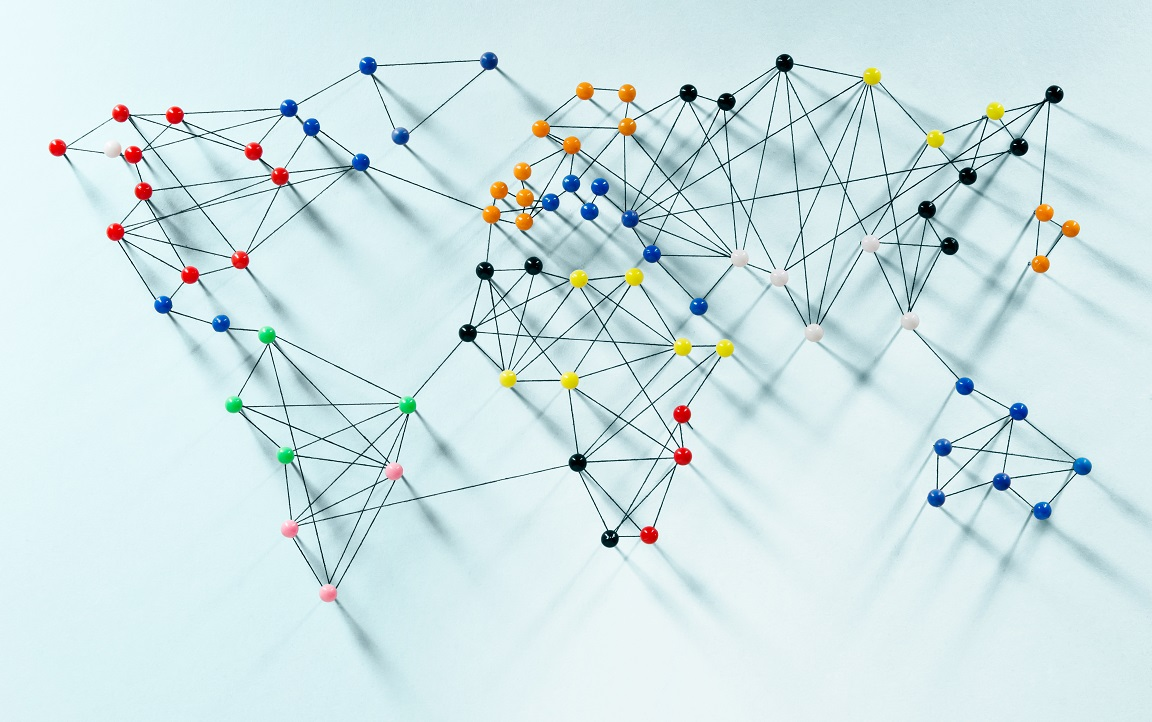
\includegraphics[scale=1]{Graph-Theory.jpg}
\caption{Grafo colorido dos continentes do planeta Terra. \cite{img:graph}}
\label{fig:graph1}
\end{figure}

\section{Relevância}
Os tópicos abordados são em sua maioria, aplicações de grafos em soluções de problemas, tais como no quesito de fluxos e optimizações. Existem muitos algoritmos de busca e optimização que são aprendidos nessa disciplina para grafos como Algoritmo de Bellman-Ford\cite{wiki:xxb} e o Algoritmo de Dijkstra\cite{wiki:xxa} que soluciona o problema do caminho mais curto num grafo. Além do problema P versus NP, que também é um problema de optimização de memória e tempo.

\section{Relação com outras cadeiras}
\subsection{IF672 - Algoritmos e Estruturas de Dados}
Na disciplina de Algoritmos e Estruturas de Dados se aprende grafo como estruturas de dados e seus algoritmos. Tais como Backtracking\cite{wiki:xxc}, o Algoritmo de Dijkstra\cite{wiki:xxa}, Algoritmo de Bellman-Ford\cite{wiki:xxb} e outros, sem um aprofundamento tão grande quanto na disciplina de Teoria dos Grafos.
\subsection{IF670 - Matemática Discreta para Computação}
Na cadeira de Matemática Discreta, se aprende a base pra manipular grafos, assim como relações entre objetos e problemas de optimização.



\bibliographystyle{plain}
\bibliography{phltc.bib}

\end{document}
